\documentclass[twoside]{book}

% Packages required by doxygen
\usepackage{fixltx2e}
\usepackage{calc}
\usepackage{doxygen}
\usepackage[export]{adjustbox} % also loads graphicx
\usepackage{graphicx}
\usepackage[utf8]{inputenc}
\usepackage{makeidx}
\usepackage{multicol}
\usepackage{multirow}
\PassOptionsToPackage{warn}{textcomp}
\usepackage{textcomp}
\usepackage[nointegrals]{wasysym}
\usepackage[table]{xcolor}

% Font selection
\usepackage[T1]{fontenc}
\usepackage[scaled=.90]{helvet}
\usepackage{courier}
\usepackage{amssymb}
\usepackage{sectsty}
\renewcommand{\familydefault}{\sfdefault}
\allsectionsfont{%
  \fontseries{bc}\selectfont%
  \color{darkgray}%
}
\renewcommand{\DoxyLabelFont}{%
  \fontseries{bc}\selectfont%
  \color{darkgray}%
}
\newcommand{\+}{\discretionary{\mbox{\scriptsize$\hookleftarrow$}}{}{}}

% Page & text layout
\usepackage{geometry}
\geometry{%
  a4paper,%
  top=2.5cm,%
  bottom=2.5cm,%
  left=2.5cm,%
  right=2.5cm%
}
\tolerance=750
\hfuzz=15pt
\hbadness=750
\setlength{\emergencystretch}{15pt}
\setlength{\parindent}{0cm}
\setlength{\parskip}{3ex plus 2ex minus 2ex}
\makeatletter
\renewcommand{\paragraph}{%
  \@startsection{paragraph}{4}{0ex}{-1.0ex}{1.0ex}{%
    \normalfont\normalsize\bfseries\SS@parafont%
  }%
}
\renewcommand{\subparagraph}{%
  \@startsection{subparagraph}{5}{0ex}{-1.0ex}{1.0ex}{%
    \normalfont\normalsize\bfseries\SS@subparafont%
  }%
}
\makeatother

% Headers & footers
\usepackage{fancyhdr}
\pagestyle{fancyplain}
\fancyhead[LE]{\fancyplain{}{\bfseries\thepage}}
\fancyhead[CE]{\fancyplain{}{}}
\fancyhead[RE]{\fancyplain{}{\bfseries\leftmark}}
\fancyhead[LO]{\fancyplain{}{\bfseries\rightmark}}
\fancyhead[CO]{\fancyplain{}{}}
\fancyhead[RO]{\fancyplain{}{\bfseries\thepage}}
\fancyfoot[LE]{\fancyplain{}{}}
\fancyfoot[CE]{\fancyplain{}{}}
\fancyfoot[RE]{\fancyplain{}{\bfseries\scriptsize Generated by Doxygen }}
\fancyfoot[LO]{\fancyplain{}{\bfseries\scriptsize Generated by Doxygen }}
\fancyfoot[CO]{\fancyplain{}{}}
\fancyfoot[RO]{\fancyplain{}{}}
\renewcommand{\footrulewidth}{0.4pt}
\renewcommand{\chaptermark}[1]{%
  \markboth{#1}{}%
}
\renewcommand{\sectionmark}[1]{%
  \markright{\thesection\ #1}%
}

% Indices & bibliography
\usepackage{natbib}
\usepackage[titles]{tocloft}
\setcounter{tocdepth}{3}
\setcounter{secnumdepth}{5}
\makeindex

% Hyperlinks (required, but should be loaded last)
\usepackage{ifpdf}
\ifpdf
  \usepackage[pdftex,pagebackref=true]{hyperref}
\else
  \usepackage[ps2pdf,pagebackref=true]{hyperref}
\fi
\hypersetup{%
  colorlinks=true,%
  linkcolor=blue,%
  citecolor=blue,%
  unicode%
}

% Custom commands
\newcommand{\clearemptydoublepage}{%
  \newpage{\pagestyle{empty}\cleardoublepage}%
}

\usepackage{caption}
\captionsetup{labelsep=space,justification=centering,font={bf},singlelinecheck=off,skip=4pt,position=top}

%===== C O N T E N T S =====

\begin{document}

% Titlepage & ToC
\hypersetup{pageanchor=false,
             bookmarksnumbered=true,
             pdfencoding=unicode
            }
\pagenumbering{alph}
\begin{titlepage}
\vspace*{7cm}
\begin{center}%
{\Large P\+U\+Ff\+Rs }\\
\vspace*{1cm}
{\large Generated by Doxygen 1.8.13}\\
\end{center}
\end{titlepage}
\clearemptydoublepage
\pagenumbering{roman}
\tableofcontents
\clearemptydoublepage
\pagenumbering{arabic}
\hypersetup{pageanchor=true}

%--- Begin generated contents ---
\chapter{Hierarchical Index}
\section{Class Hierarchy}
This inheritance list is sorted roughly, but not completely, alphabetically\+:\begin{DoxyCompactList}
\item \contentsline{section}{puffrs\+:\+:Discretization}{\pageref{classpuffrs_1_1Discretization}}{}
\begin{DoxyCompactList}
\item \contentsline{section}{puffrs\+:\+:Regular\+Discretization}{\pageref{classpuffrs_1_1RegularDiscretization}}{}
\end{DoxyCompactList}
\item \contentsline{section}{puffrs\+:\+:Discretization\+Factory}{\pageref{classpuffrs_1_1DiscretizationFactory}}{}
\item \contentsline{section}{puffrs\+:\+:Puffrs}{\pageref{classpuffrs_1_1Puffrs}}{}
\item \contentsline{section}{puffrs\+:\+:Puffrs\+Factory}{\pageref{classpuffrs_1_1PuffrsFactory}}{}
\item \contentsline{section}{puffrs\+:\+:Puffrs\+Parser}{\pageref{classpuffrs_1_1PuffrsParser}}{}
\end{DoxyCompactList}

\chapter{Class Index}
\section{Class List}
Here are the classes, structs, unions and interfaces with brief descriptions\+:\begin{DoxyCompactList}
\item\contentsline{section}{\hyperlink{classpuffrs_1_1Discretization}{puffrs\+::\+Discretization} }{\pageref{classpuffrs_1_1Discretization}}{}
\item\contentsline{section}{\hyperlink{classpuffrs_1_1DiscretizationFactory}{puffrs\+::\+Discretization\+Factory} }{\pageref{classpuffrs_1_1DiscretizationFactory}}{}
\item\contentsline{section}{\hyperlink{classpuffrs_1_1Puffrs}{puffrs\+::\+Puffrs} }{\pageref{classpuffrs_1_1Puffrs}}{}
\item\contentsline{section}{\hyperlink{classpuffrs_1_1PuffrsFactory}{puffrs\+::\+Puffrs\+Factory} }{\pageref{classpuffrs_1_1PuffrsFactory}}{}
\item\contentsline{section}{\hyperlink{classpuffrs_1_1PuffrsParser}{puffrs\+::\+Puffrs\+Parser} }{\pageref{classpuffrs_1_1PuffrsParser}}{}
\item\contentsline{section}{\hyperlink{classpuffrs_1_1RegularDiscretization}{puffrs\+::\+Regular\+Discretization} \\*Discretiation class for regular discretization }{\pageref{classpuffrs_1_1RegularDiscretization}}{}
\end{DoxyCompactList}

\chapter{Class Documentation}
\hypertarget{classpuffrs_1_1Discretization}{}\section{puffrs\+:\+:Discretization Class Reference}
\label{classpuffrs_1_1Discretization}\index{puffrs\+::\+Discretization@{puffrs\+::\+Discretization}}


Inheritance diagram for puffrs\+:\+:Discretization\+:

\hypertarget{classpuffrs_1_1DiscretizationFactory}{}\section{puffrs\+:\+:Discretization\+Factory Class Reference}
\label{classpuffrs_1_1DiscretizationFactory}\index{puffrs\+::\+Discretization\+Factory@{puffrs\+::\+Discretization\+Factory}}
\subsection*{Public Member Functions}
\begin{DoxyCompactItemize}
\item 
\mbox{\Hypertarget{classpuffrs_1_1DiscretizationFactory_af6d6e4dfb783d8a85208680f84e50cda}\label{classpuffrs_1_1DiscretizationFactory_af6d6e4dfb783d8a85208680f84e50cda}} 
\hyperlink{classpuffrs_1_1DiscretizationFactory_af6d6e4dfb783d8a85208680f84e50cda}{Discretization\+Factory} (const Teuchos\+::\+R\+CP$<$ Teuchos\+::\+Parameter\+List $>$ \&k\+Discretization\+Parameters)
\begin{DoxyCompactList}\small\item\em Default constructor. \end{DoxyCompactList}\item 
\mbox{\Hypertarget{classpuffrs_1_1DiscretizationFactory_a179e7c336204e55c07de5510398b090a}\label{classpuffrs_1_1DiscretizationFactory_a179e7c336204e55c07de5510398b090a}} 
virtual Teuchos\+::\+R\+CP$<$ \hyperlink{classpuffrs_1_1Discretization}{Discretization} $>$ {\bfseries Create} (const Teuchos\+::\+R\+CP$<$ const Teuchos\+::\+Comm$<$ types\+::\+Puffrs\+Comm $>$ $>$ \&k\+Comm)
\end{DoxyCompactItemize}
\subsection*{Protected Attributes}
\begin{DoxyCompactItemize}
\item 
\mbox{\Hypertarget{classpuffrs_1_1DiscretizationFactory_a5375e76d7af9c10d52eb374ead8a922c}\label{classpuffrs_1_1DiscretizationFactory_a5375e76d7af9c10d52eb374ead8a922c}} 
const Teuchos\+::\+R\+CP$<$ Teuchos\+::\+Parameter\+List $>$ \hyperlink{classpuffrs_1_1DiscretizationFactory_a5375e76d7af9c10d52eb374ead8a922c}{k\+Discretization\+Parameters\+\_\+}
\begin{DoxyCompactList}\small\item\em Parameter list. \end{DoxyCompactList}\end{DoxyCompactItemize}


The documentation for this class was generated from the following files\+:\begin{DoxyCompactItemize}
\item 
src/puffrs\+\_\+discretization\+\_\+factory.\+h\item 
src/puffrs\+\_\+discretization\+\_\+factory.\+cc\end{DoxyCompactItemize}

\hypertarget{classpuffrs_1_1Puffrs}{}\section{puffrs\+:\+:Puffrs Class Reference}
\label{classpuffrs_1_1Puffrs}\index{puffrs\+::\+Puffrs@{puffrs\+::\+Puffrs}}
\subsection*{Public Member Functions}
\begin{DoxyCompactItemize}
\item 
\mbox{\Hypertarget{classpuffrs_1_1Puffrs_abcef5a8b8844d979db872e51b8f89abb}\label{classpuffrs_1_1Puffrs_abcef5a8b8844d979db872e51b8f89abb}} 
{\bfseries Puffrs} (const Teuchos\+::\+R\+CP$<$ const Teuchos\+::\+Comm$<$ int $>$ $>$ \&k\+Comm, Teuchos\+::\+R\+CP$<$ Teuchos\+::\+Parameter\+List $>$ parameters, Teuchos\+::\+R\+CP$<$ \hyperlink{classpuffrs_1_1Discretization}{puffrs\+::\+Discretization} $>$ puffrs\+\_\+discretization)
\end{DoxyCompactItemize}


The documentation for this class was generated from the following files\+:\begin{DoxyCompactItemize}
\item 
src/puffrs.\+h\item 
src/puffrs.\+cc\end{DoxyCompactItemize}

\hypertarget{classpuffrs_1_1PuffrsFactory}{}\section{puffrs\+:\+:Puffrs\+Factory Class Reference}
\label{classpuffrs_1_1PuffrsFactory}\index{puffrs\+::\+Puffrs\+Factory@{puffrs\+::\+Puffrs\+Factory}}
\subsection*{Public Member Functions}
\begin{DoxyCompactItemize}
\item 
\mbox{\Hypertarget{classpuffrs_1_1PuffrsFactory_a1b0f9bebc29e95a6e02a0a10d33d378c}\label{classpuffrs_1_1PuffrsFactory_a1b0f9bebc29e95a6e02a0a10d33d378c}} 
virtual Teuchos\+::\+R\+CP$<$ \hyperlink{classpuffrs_1_1Puffrs}{puffrs\+::\+Puffrs} $>$ {\bfseries Create} (const std\+::string k\+Input\+File, const Teuchos\+::\+R\+CP$<$ const Teuchos\+::\+Comm$<$ types\+::\+Puffrs\+Comm $>$ $>$ \&k\+Comm, Teuchos\+::\+R\+CP$<$ \hyperlink{classpuffrs_1_1Discretization}{puffrs\+::\+Discretization} $>$ puffrs\+\_\+discretization)
\item 
\mbox{\Hypertarget{classpuffrs_1_1PuffrsFactory_aaa29b92655e69498acaac735b673b409}\label{classpuffrs_1_1PuffrsFactory_aaa29b92655e69498acaac735b673b409}} 
virtual Teuchos\+::\+R\+CP$<$ \hyperlink{classpuffrs_1_1Puffrs}{puffrs\+::\+Puffrs} $>$ {\bfseries Create} (const std\+::string k\+Input\+File, const Teuchos\+::\+R\+CP$<$ const Teuchos\+::\+Comm$<$ types\+::\+Puffrs\+Comm $>$ $>$ \&k\+Comm)
\end{DoxyCompactItemize}


The documentation for this class was generated from the following file\+:\begin{DoxyCompactItemize}
\item 
src/puffrs\+\_\+factory.\+h\end{DoxyCompactItemize}

\hypertarget{classpuffrs_1_1PuffrsParser}{}\section{puffrs\+:\+:Puffrs\+Parser Class Reference}
\label{classpuffrs_1_1PuffrsParser}\index{puffrs\+::\+Puffrs\+Parser@{puffrs\+::\+Puffrs\+Parser}}
\subsection*{Static Public Member Functions}
\begin{DoxyCompactItemize}
\item 
static Teuchos\+::\+R\+CP$<$ Teuchos\+::\+Parameter\+List $>$ \hyperlink{classpuffrs_1_1PuffrsParser_aa41312817bfa20dc93e80790f51a720b}{Parse} (const std\+::string k\+Input\+File)
\end{DoxyCompactItemize}


\subsection{Member Function Documentation}
\mbox{\Hypertarget{classpuffrs_1_1PuffrsParser_aa41312817bfa20dc93e80790f51a720b}\label{classpuffrs_1_1PuffrsParser_aa41312817bfa20dc93e80790f51a720b}} 
\index{puffrs\+::\+Puffrs\+Parser@{puffrs\+::\+Puffrs\+Parser}!Parse@{Parse}}
\index{Parse@{Parse}!puffrs\+::\+Puffrs\+Parser@{puffrs\+::\+Puffrs\+Parser}}
\subsubsection{\texorpdfstring{Parse()}{Parse()}}
{\footnotesize\ttfamily Teuchos\+::\+R\+CP$<$ Teuchos\+::\+Parameter\+List $>$ puffrs\+::\+Puffrs\+Parser\+::\+Parse (\begin{DoxyParamCaption}\item[{const std\+::string}]{k\+Input\+File }\end{DoxyParamCaption})\hspace{0.3cm}{\ttfamily [static]}}

With a little bit of a elaboration, should you feel it necessary. 
\begin{DoxyParams}{Parameters}
{\em k\+Input\+File} & ... File Parser ... \\
\hline
\end{DoxyParams}


The documentation for this class was generated from the following files\+:\begin{DoxyCompactItemize}
\item 
src/puffrs\+\_\+parser.\+h\item 
src/puffrs\+\_\+parser.\+cc\end{DoxyCompactItemize}

\hypertarget{classpuffrs_1_1RegularDiscretization}{}\section{puffrs\+:\+:Regular\+Discretization Class Reference}
\label{classpuffrs_1_1RegularDiscretization}\index{puffrs\+::\+Regular\+Discretization@{puffrs\+::\+Regular\+Discretization}}


Discretiation class for regular discretization.  




{\ttfamily \#include $<$puffrs\+\_\+regular\+\_\+discretization.\+h$>$}



Inheritance diagram for puffrs\+:\+:Regular\+Discretization\+:
\nopagebreak
\begin{figure}[H]
\begin{center}
\leavevmode
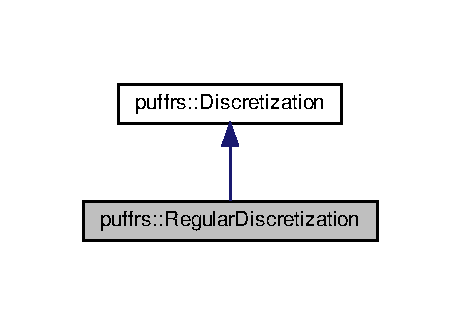
\includegraphics[width=221pt]{classpuffrs_1_1RegularDiscretization__inherit__graph}
\end{center}
\end{figure}


Collaboration diagram for puffrs\+:\+:Regular\+Discretization\+:
\nopagebreak
\begin{figure}[H]
\begin{center}
\leavevmode
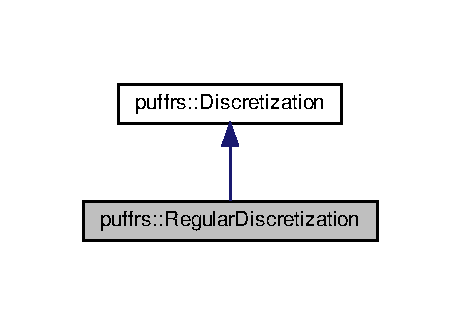
\includegraphics[width=221pt]{classpuffrs_1_1RegularDiscretization__coll__graph}
\end{center}
\end{figure}
\subsection*{Public Member Functions}
\begin{DoxyCompactItemize}
\item 
\mbox{\Hypertarget{classpuffrs_1_1RegularDiscretization_adb66672889168f2829fd7d8b1cc5faee}\label{classpuffrs_1_1RegularDiscretization_adb66672889168f2829fd7d8b1cc5faee}} 
{\bfseries Regular\+Discretization} (const Teuchos\+::\+R\+CP$<$ const Teuchos\+::\+Comm$<$ int $>$ $>$ \&k\+Comm, const Teuchos\+::\+R\+CP$<$ Teuchos\+::\+Parameter\+List $>$ \&k\+Discretization\+Parameters)
\end{DoxyCompactItemize}
\subsection*{Protected Attributes}
\begin{DoxyCompactItemize}
\item 
\mbox{\Hypertarget{classpuffrs_1_1RegularDiscretization_a5306dd2eda5b9c75850e889e6b0a2b54}\label{classpuffrs_1_1RegularDiscretization_a5306dd2eda5b9c75850e889e6b0a2b54}} 
const Teuchos\+::\+R\+CP$<$ const Teuchos\+::\+Comm$<$ int $>$ $>$ \& {\bfseries k\+Comm\+\_\+}
\end{DoxyCompactItemize}
\subsection*{Additional Inherited Members}


\subsection{Detailed Description}
Discretiation class for regular discretization. 

The documentation for this class was generated from the following file\+:\begin{DoxyCompactItemize}
\item 
src/puffrs\+\_\+regular\+\_\+discretization.\+h\end{DoxyCompactItemize}

%--- End generated contents ---

% Index
\backmatter
\newpage
\phantomsection
\clearemptydoublepage
\addcontentsline{toc}{chapter}{Index}
\printindex

\end{document}
